\documentclass[UTF8,a4paper,zihao=-4]{ctexart}

\usepackage[margin=2.4cm]{geometry}
\usepackage{graphicx}
\usepackage{booktabs}
\usepackage{amsmath}
\usepackage{array}
\usepackage{float}
\usepackage{caption}
\usepackage{enumitem}
\usepackage{tikz}
\usetikzlibrary{arrows.meta,positioning,fit,backgrounds}
\usepackage[hidelinks]{hyperref}

\captionsetup{font=small,labelsep=quad}
\setlist{nosep,leftmargin=2em}
\renewcommand{\arraystretch}{1.25}
\hyphenation{Revit BIM HVACIDA}
\tolerance=3000
\emergencystretch=3em

\title{\heiti 从公式文档到设计交付:\\地铁暖通 BIM 正向设计工具链的构建}
\author{韩学伟\\[2pt] \small 中铁第六勘察设计院集团有限公司电气化设计院分公司,天津}
\date{}

\begin{document}
\maketitle

\begin{abstract}
\noindent
地铁车站暖通设计由取数、计算、选型、统计与出图多段工作拼成,实际生产中往往退化为若干互不相通的"点工具":Excel 算负荷、插件算排烟、人工整理计算书。本文把这条作业链作为一个整体来构建,提出一条由五个环节组成的正向设计工具链:规则建模、模型取值、计算内核、一致输出、交付生成,并用数据约定与三道自动检查把环节串起来。工具链在 Revit 2020 上实现为 7 个面板、24 个按钮的插件,包含大系统负荷与排烟、六类小系统、风/水系统水力、材料表与图框。北京站算例给出总制冷量 381.598 kW、总送风量 87\,768 m$^3$/h,六类小系统示例逐格复算一致;900 余条数值断言与窗口装载自检保证改动不破坏规则。文章最后讨论了工具链的瓶颈在规则而不在算法、输出一致是交付的验收条件这两个判断,并说明迁移成本与局限。
\vspace{0.5em}

\noindent\textbf{关键词:} BIM 正向设计;工具链;地铁车站;暖通空调;Revit 二次开发;数据约定
\end{abstract}

\section{引言}

设计院里的暖通设计并不缺"能算的地方"。负荷可以用 Excel 算,排烟可以查表,选型可以翻样本,图纸可以用 Revit 出。缺的是把这些"能算的地方"连起来的东西:一个房间的面积在模型里量一次,却要在三张表里抄三遍;一份公式在文档里改一行,要在五处代码里跟着改;一张计算书交付出去,评审问"这个数怎么来的",设计人只能翻聊天记录。

这类问题常被归为"效率",但根子在\emph{接口}。当每一段工作都有独立的输入输出、彼此靠人工转录衔接时,任何一段变动都会在链上放大:面积改一次,负荷、选型、材料表、计算书全要重做;而每一处重做都可能引入新错误。本文把这条作业链作为一个整体来设计,称之为\textbf{正向设计工具链},并用一套可运行的软件把它落下来。

需要区分的是"点工具"与"工具链":点工具解决某一个环节的自动化,工具链解决环节之间的传递。点工具做得好,能省掉一段人工;工具链做得好,能让改动只发生一次。后者更接近设计院对"正向设计"的期待——模型改,成果跟着改,而不是模型改完再重做一轮成果。

本文的结构:第 2 节给出工具链的五个环节与两条贯穿线;第 3 节逐段说明实现;第 4 节讨论贯通性(数据约定与自动检查);第 5 节给出工程应用与验证;第 6 节讨论工具链的瓶颈、一致交付与迁移成本;第 7 节总结。

\section{工具链的总体设计}

\subsection{五个环节}

工具链由五个环节组成(图\ref{fig:chain}):\textbf{规则建模}把院内的公式文档解析成可执行的规格;\textbf{模型取值}从 Revit 空间、墙体、图纸中取出几何与清单;\textbf{计算内核}按规格算出六类小系统、大系统与水力结果;\textbf{一致输出}把结果组织成一份对象,再分别渲染为界面、文本与 Excel;\textbf{交付生成}输出计算书、材料表与图册。每个环节的输入输出都是显式定义的(表\ref{tab:stages}),上一段的输出就是下一段的约定。

\begin{figure}[H]
\centering
\resizebox{0.98\textwidth}{!}{%
\begin{tikzpicture}[
  st/.style={draw,rounded corners=2pt,minimum height=1.15cm,text width=2.45cm,align=center,font=\small},
  arr/.style={-{Stealth[length=2mm]},thick},
  gate/.style={draw,dashed,rounded corners=3pt,fill=gray!6,minimum height=0.9cm,text width=12.4cm,align=center,font=\small}
]
\node[st,fill=blue!7] (s1) {1. 规则建模\\公式文档 → 规格};
\node[st,fill=blue!7,right=0.35cm of s1] (s2) {2. 模型取值\\空间/墙体/图纸};
\node[st,fill=green!7,right=0.35cm of s2] (s3) {3. 计算内核\\六类 + 大系统 + 水力};
\node[st,fill=orange!9,right=0.35cm of s3] (s4) {4. 一致输出\\界面/文本/Excel};
\node[st,fill=gray!9,right=0.35cm of s4] (s5) {5. 交付生成\\计算书/材料表/图册};
\node[gate,below=0.95cm of s3] (g) {三道自动检查:数值断言(900+) · 窗口装载自检(190+) · 结构自检(7 面板/24 按钮)};
\foreach \s in {s1,s2,s3,s4,s5} { \draw[arr,dashed,gray] (\s.south) -- (g.north); }
\draw[arr] (s1) -- (s2); \draw[arr] (s2) -- (s3);
\draw[arr] (s3) -- (s4); \draw[arr] (s4) -- (s5);
\end{tikzpicture}}
\caption{正向设计工具链:五个环节与贯穿的自动检查}\label{fig:chain}
\end{figure}

\begin{table}[H]
\centering
\caption{工具链各环节的输入、输出与交付物}\label{tab:stages}
\small
\begin{tabular}{p{2.4cm}p{4.6cm}p{4.4cm}p{3.6cm}}
\toprule
环节 & 输入 & 输出 & 对应交付物 \\
\midrule
规则建模 & 院内公式文档、算例 & 常量、公式、默认值、校核值 & 规则说明(计算书附页) \\
模型取值 & Revit 空间/墙体/图纸 & 带来源 Id 的几何量与清单 & 房间表、图纸清单 \\
计算内核 & 参数 + 几何 & 逐房间与系统级结果对象 & 无(纯计算) \\
一致输出 & 结果对象 & 界面表格、文本、Excel & 三处同数 \\
交付生成 & 结果 + 清单 & 计算书、材料表、图册 & 出图与归档 \\
\bottomrule
\end{tabular}
\end{table}

\subsection{两条贯穿线:数据约定与自动检查}

工具链最容易断的地方不在两端,而在中间:一段的输出格式变了,下一段悄悄读错,最后表现为"数不对"。为此设了两条贯穿线。

\textbf{数据约定}。所有跨环节的数据都有明确载体:计算输入是 \texttt{SmallSystemInput}、\texttt{LargeSystemInput} 等模型类,计算结果是对应的 \texttt{Result} 类,交付件只从 \texttt{ResultTable} 读;落盘统一为 XML,字段增删必须同时改读取端。约定不写进散文,而是写进类型——编译器与自检替人看守。

\textbf{三道自动检查}。数值(900 余条断言)、界面(12 个窗口约 450 个绑定、190 余项)、结构(7 面板/24 按钮/48 张图标)在每次提交前运行,失败即阻断(表\ref{tab:gates})。自动检查不是"测试覆盖率"的数字游戏,而是把"这次改动有没有破坏上一段的约定"变成一条命令能回答的问题。

\begin{table}[H]
\centering
\caption{三道提交前自动检查}\label{tab:gates}
\small
\begin{tabular}{p{3.0cm}p{6.2cm}p{3.2cm}p{2.2cm}}
\toprule
自动检查 & 覆盖内容 & 规模 & 失败处理 \\
\midrule
计算内核自检 & 大系统负荷/排烟、六类小系统、气象库、水力、材料表、知识库 & 900+ 条断言 & 阻断提交 \\
窗口装载自检 & 12 个窗口、约 450 个数据绑定、按钮与保存行为 & 190+ 项 & 阻断提交 \\
功能区自检 & 7 面板 / 24 按钮 / 16·32 像素图标 & 24 组图标 & 阻断提交 \\
\bottomrule
\end{tabular}
\end{table}

\section{关键环节的实现}

\subsection{规则建模:从公式文档到可执行规格}

规则建模是工具链的第一环,也是决定上限的一环。院内公式文档是给人看的:量用单元格代号标识,系数散落在文字里,示例与正文偶有不一致。把它变成可执行规格,需要三件事:量有名字、系数有出处、结果有校核值(表\ref{tab:formula})。

\begin{table}[H]
\centering
\caption{多联机+新风公式链的文档—代码—校核值对照(示例 7 房间)}\label{tab:formula}
\footnotesize
\begin{tabular}{p{3.1cm}p{5.6cm}p{4.1cm}}
\toprule
计算量 & 代码实现(节选) & 示例校核值 \\
\midrule
房间冷负荷 & \texttt{SmallRoomResult.TotalCoolingKw} & 1.888 kW \\
消除余热通风量 & \texttt{HeatVentilationM3H} & 431.3785 m³/h \\
计算通风量 & \texttt{ActualVentilationM3H} & 431.3785 m³/h \\
新风冷负荷 & \texttt{UnitCoolingKw} & 0.5012 kW \\
单台计算/选型冷量 & \texttt{UnitCalcCoolingKw} / \texttt{UnitSelectCoolingKw} & 2.0768 / 2.8 kW \\
房间选型冷量 & \texttt{RoomSelectCoolingKw} & 2.8 kW \\
室外机选型冷量 & \texttt{OutdoorUnitSelectCoolingKw} & 27.3184 kW \\
\bottomrule
\end{tabular}
\end{table}

移植遵循三条约束:逐式对应(方法注释标出文档位置)、不发明系数(文档未给的量不外推,确需补全时写进规则说明)、示例只用于理解(示例作回归输入,不作规则来源)。三条约束里最容易被忽视的是第三条:当示例与正文冲突时,以正文为准并显式记录差异,比"挑一个能对上示例的实现"更安全——后者会让下一位维护者无从判断。

\subsection{模型取值:空间、墙体与图纸}

模型取值把 Revit 里的对象变成工具链能用的数。这里有两个工程细节值得记录。其一是类型陷阱:Revit 2020 的空间属于"存在于 API、不在原生对象模型"的类型,按类型过滤会抛异常,必须先按 \texttt{SpatialElement} 收集再筛 \texttt{Space};这类错误编译期不报、运行期才炸,所以自动检查里加了静态扫描,禁止该写法回归。

其二是取值的时效性。房间行记录来源空间 Id,每次开窗按 Id 重读模型的面积与层高:模型改了,表里的几何量随之更新;空间被删除时保留上次的值并提示。几何量统一保留 1 位小数,且"界面显示位数 = 参与计算位数",避免"表里 4.55、算的时候 4.547"的隐性偏差。外墙长度不在空间属性里,改用两点测量在模型中直接量距,结果写入选中行。

\subsection{计算内核:不依赖 Revit 的可测实现}

计算内核放在 Core 程序集,不引用 Revit API,因此可以在没有 Revit 的环境里跑单元级回归。这一决定贯穿工具链:六类小系统、大系统负荷、排烟、水力都只吃模型类、吐结果类,与界面和 Revit 无关。好处有三:回归跑得快(纯内存计算)、规则争议可以脱离软件讨论、同一内核可被计算书与 Excel 复用。

以多联机+新风为例,内核逐房间算出冷负荷、消除余热通风量、计算通风量、新风冷负荷与室内机选型,再汇总出新风机组、送排风机与室外机的选型值;其中的系数(1.1 选型、1.15 管道附加、1.2 密度)都是带出处的常量,任何改动都会在断言里立刻显形。

\subsection{一致输出:一份结果、三处呈现}

一致输出是工具链的"腰部":它把内核的结果组织成与界面无关的结果表对象(分节、行、单位、小数位),再由三个渲染器分别输出界面表格、文本计算书与 Excel(图\ref{fig:pipeline})。三者读同一份对象,因此不会出现"界面一个数、计算书另一个数"。

\begin{figure}[H]
\centering
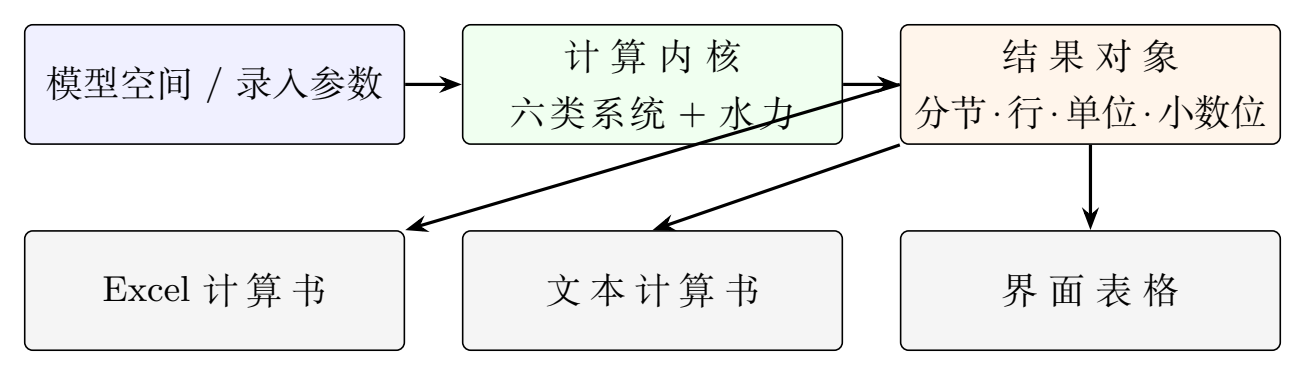
\includegraphics[width=0.93\textwidth]{figures/fig-pipeline.png}
\caption{一次计算、三处呈现:结果对象与三个渲染器}\label{fig:pipeline}
\end{figure}

Excel 计算书由自写的 XLSX 写入器生成(直接拼装 ZIP 与 XML 部件),不依赖第三方库。小系统单套计算书包含计算参数、系统结果、房间明细(带合计行)、设备选型、说明与待补五页;房间明细的列定义与界面参考表共用同一份元数据,列名、顺序与小数位不会分叉。

\subsection{交付生成:计算书、材料表与图册}

交付是工具链的终点,也是验收的起点。计算书之外,材料表按"类别 + 族 + 类型 + 单位"归并,单位进入归并键,长度与件数不互相求和;图框模块读取模型中的图纸,列出编号、名称、图框类型、图幅、视图数与是否空图框,支持按 DWG/DXF 逐张导出、PDF 走系统打印机,并在平面视图中批量标注空间名称与编号(图\ref{fig:sheets})。

\begin{figure}[H]
\centering
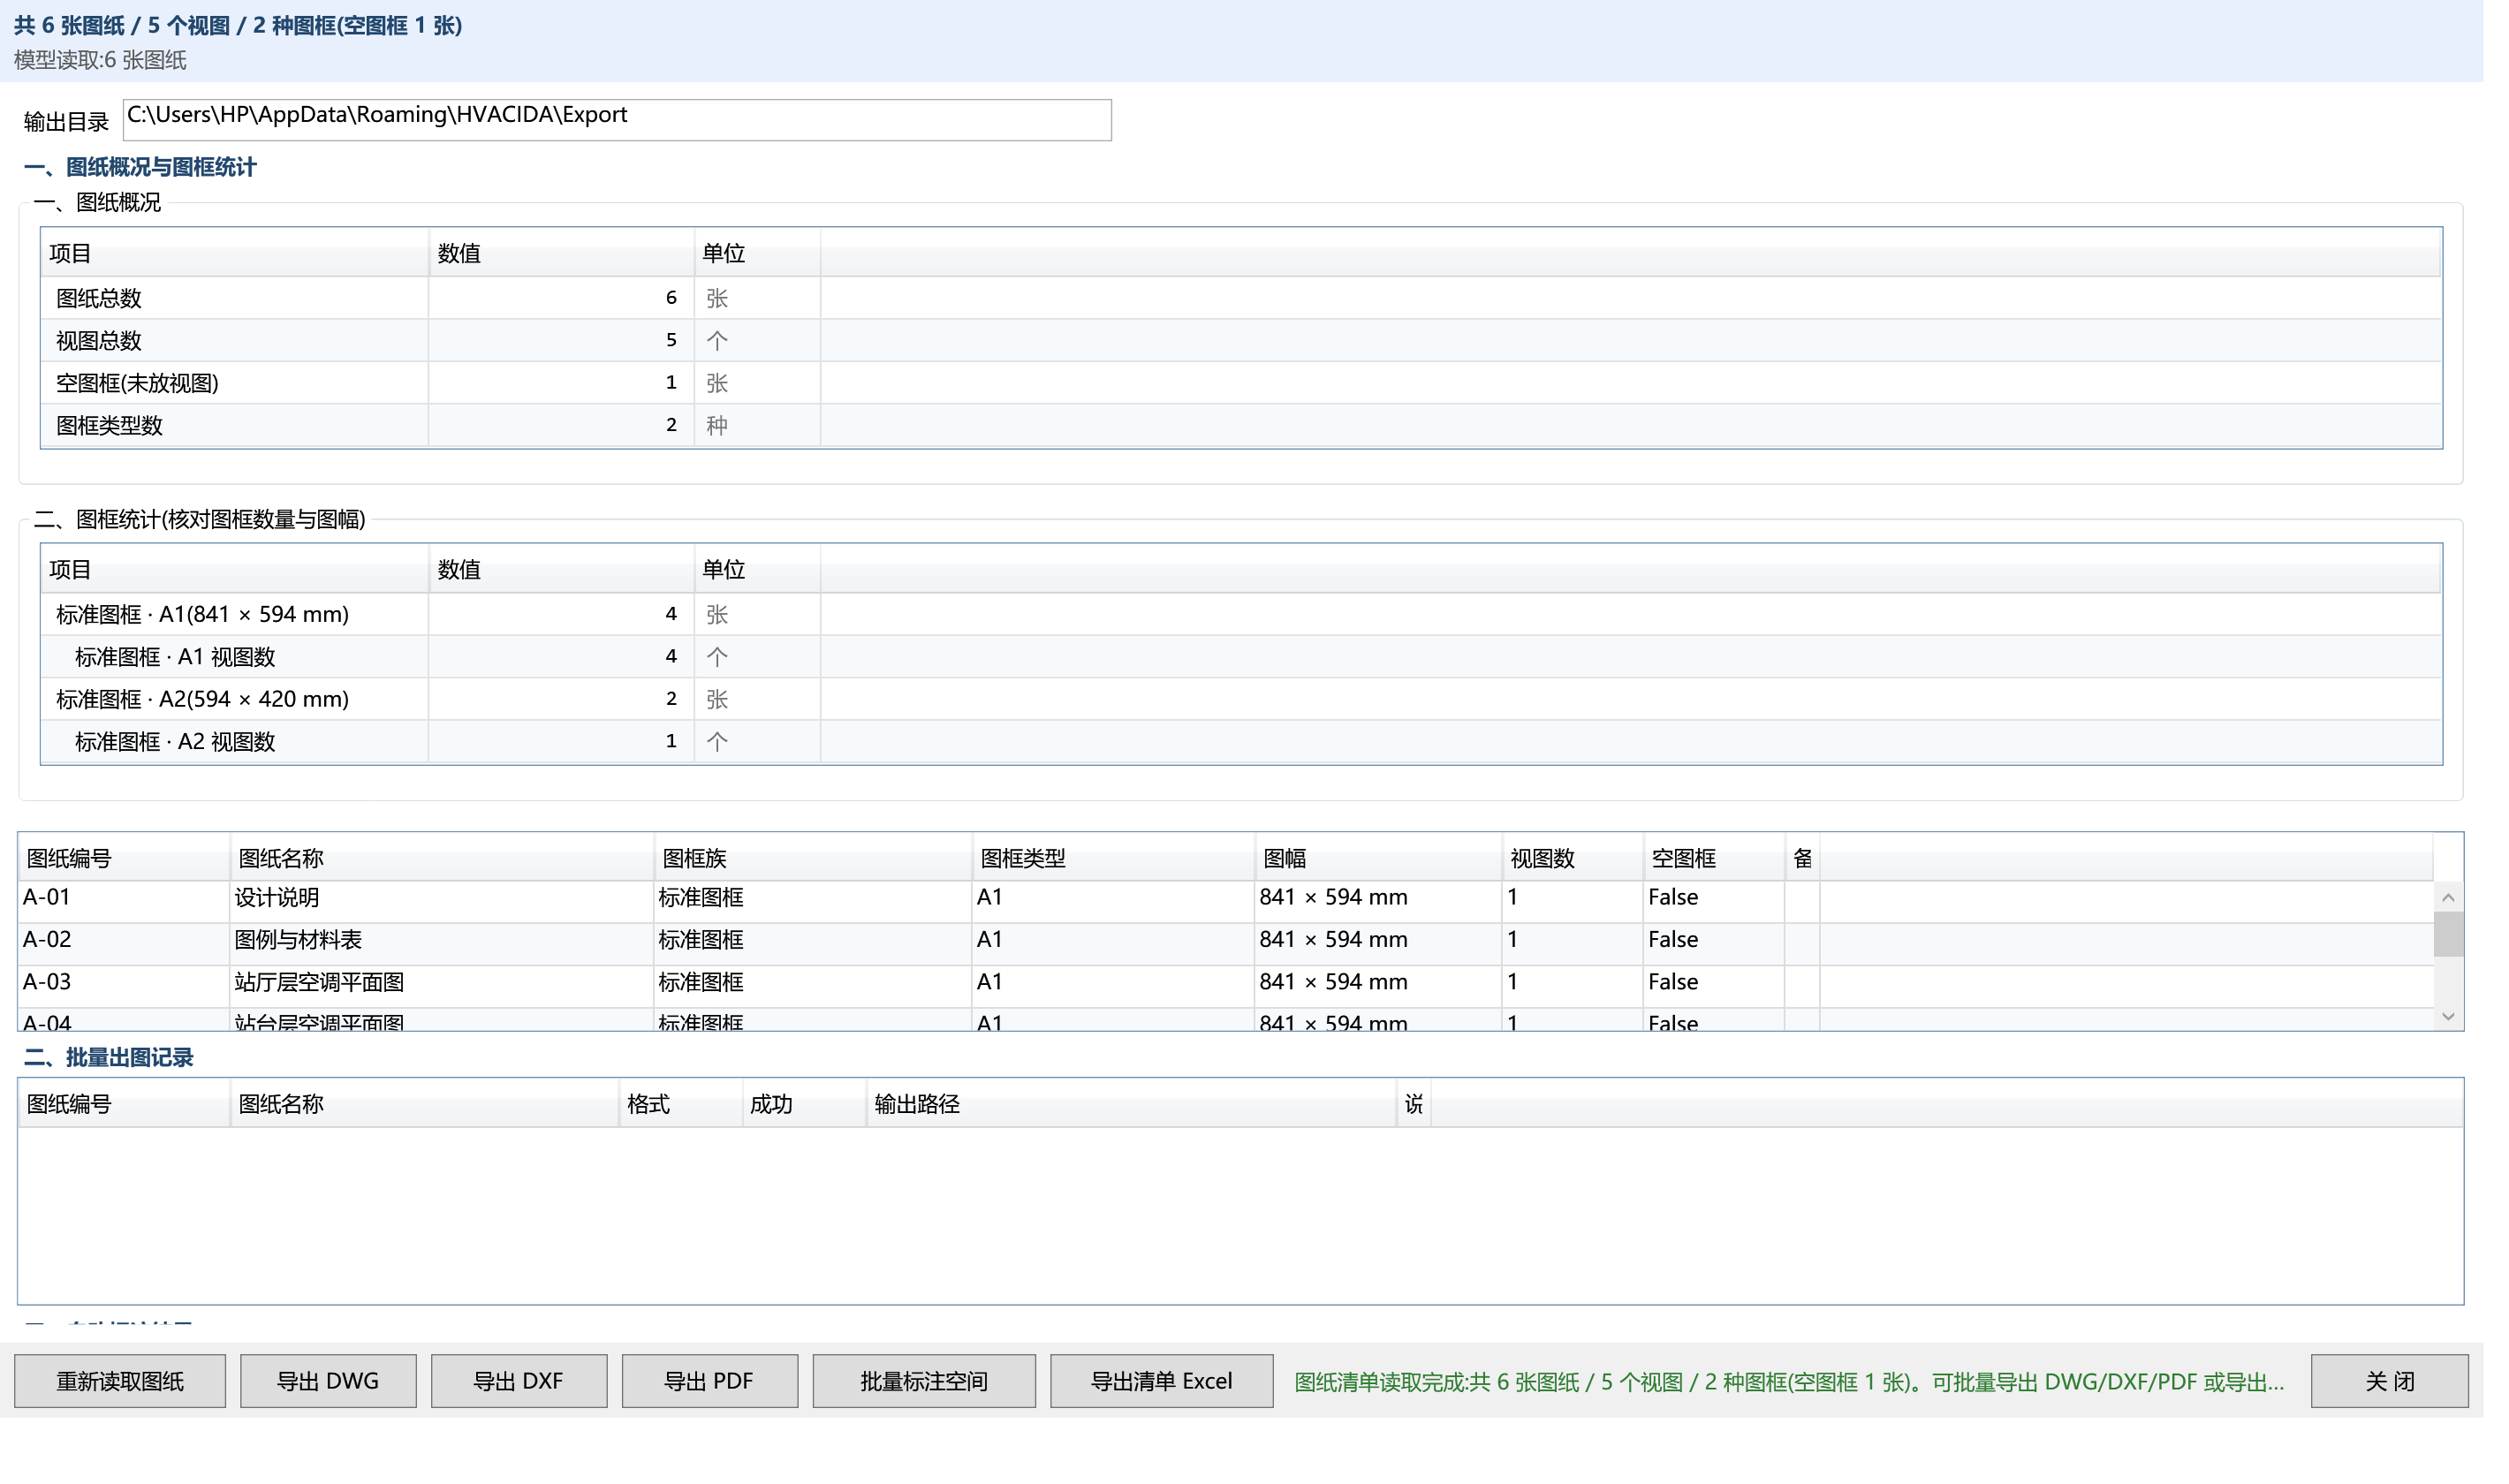
\includegraphics[width=0.95\textwidth]{figures/sheets.png}
\caption{图框窗:图纸清单与批量出图记录}\label{fig:sheets}
\end{figure}

\section{工具链的贯通性}

\subsection{数据约定}

跨环节的数据约定分为三层。第一层是\textbf{模型类}:输入侧有 \texttt{SmallSystemInput}、\texttt{SmallRoomInput}、\texttt{LargeSystemInput}、\texttt{HydraulicInput},输出侧有对应的 \texttt{Result};字段名与含义在类注释里写死,增删字段必须同步改读取端。第二层是\textbf{结果表}:界面、文本、Excel 都只认 \texttt{ResultTable},它规定分节、行、单位与小数位。第三层是\textbf{落盘格式}:工程、大系统、小系统、水力各一个 XML,旧版单系统文件在首次读取时自动迁移。

约定的价值在变动时才显现。加一个"室内机台数"字段,要改的是:输入类、结果类、计算器、房间表列定义、Excel 导出、界面绑定与断言;只要有一处漏改,自动检查会在几分钟内指出来。没有约定与自动检查时,这类改动靠人工过一遍六个窗口,漏一处就等到交付前才发现。

\subsection{自动检查的成本与收益}

写一条断言的成本与移植一条公式相当,看起来是"多花一倍时间"。但断言是可复用的:本项目累计 112 次提交,900 余条断言在每次改动上重复运行,单次成本早已被摊薄。更重要的是,自动检查把"这次改动有没有破坏上一段的约定"从经验判断变成命令输出,让工具链的维护不必依赖某一个人的记忆。

\section{应用与验证}

\subsection{工程应用}

以某地铁车站为例:站厅公共区 2\,860 m$^2$、站台公共区 1\,980 m$^2$,设 8 个设备管理用房。设计人在公共区参数窗完成空间识别与客流录入后,大系统负荷计算窗按 7 个分区录入围护结构、客流、照明、设备与新风参数,计算结果窗给出计算参数与选型参数两段(图\ref{fig:calc})。小系统按房间类型分别建立全空气一次回风与多联机+新风系统,房间表按参考表列出每个房间的逐项计算值(图\ref{fig:vrf}),设计人只需维护面积、人数、设备冷负荷与选型冷量等少量输入。

\begin{figure}[H]
\centering
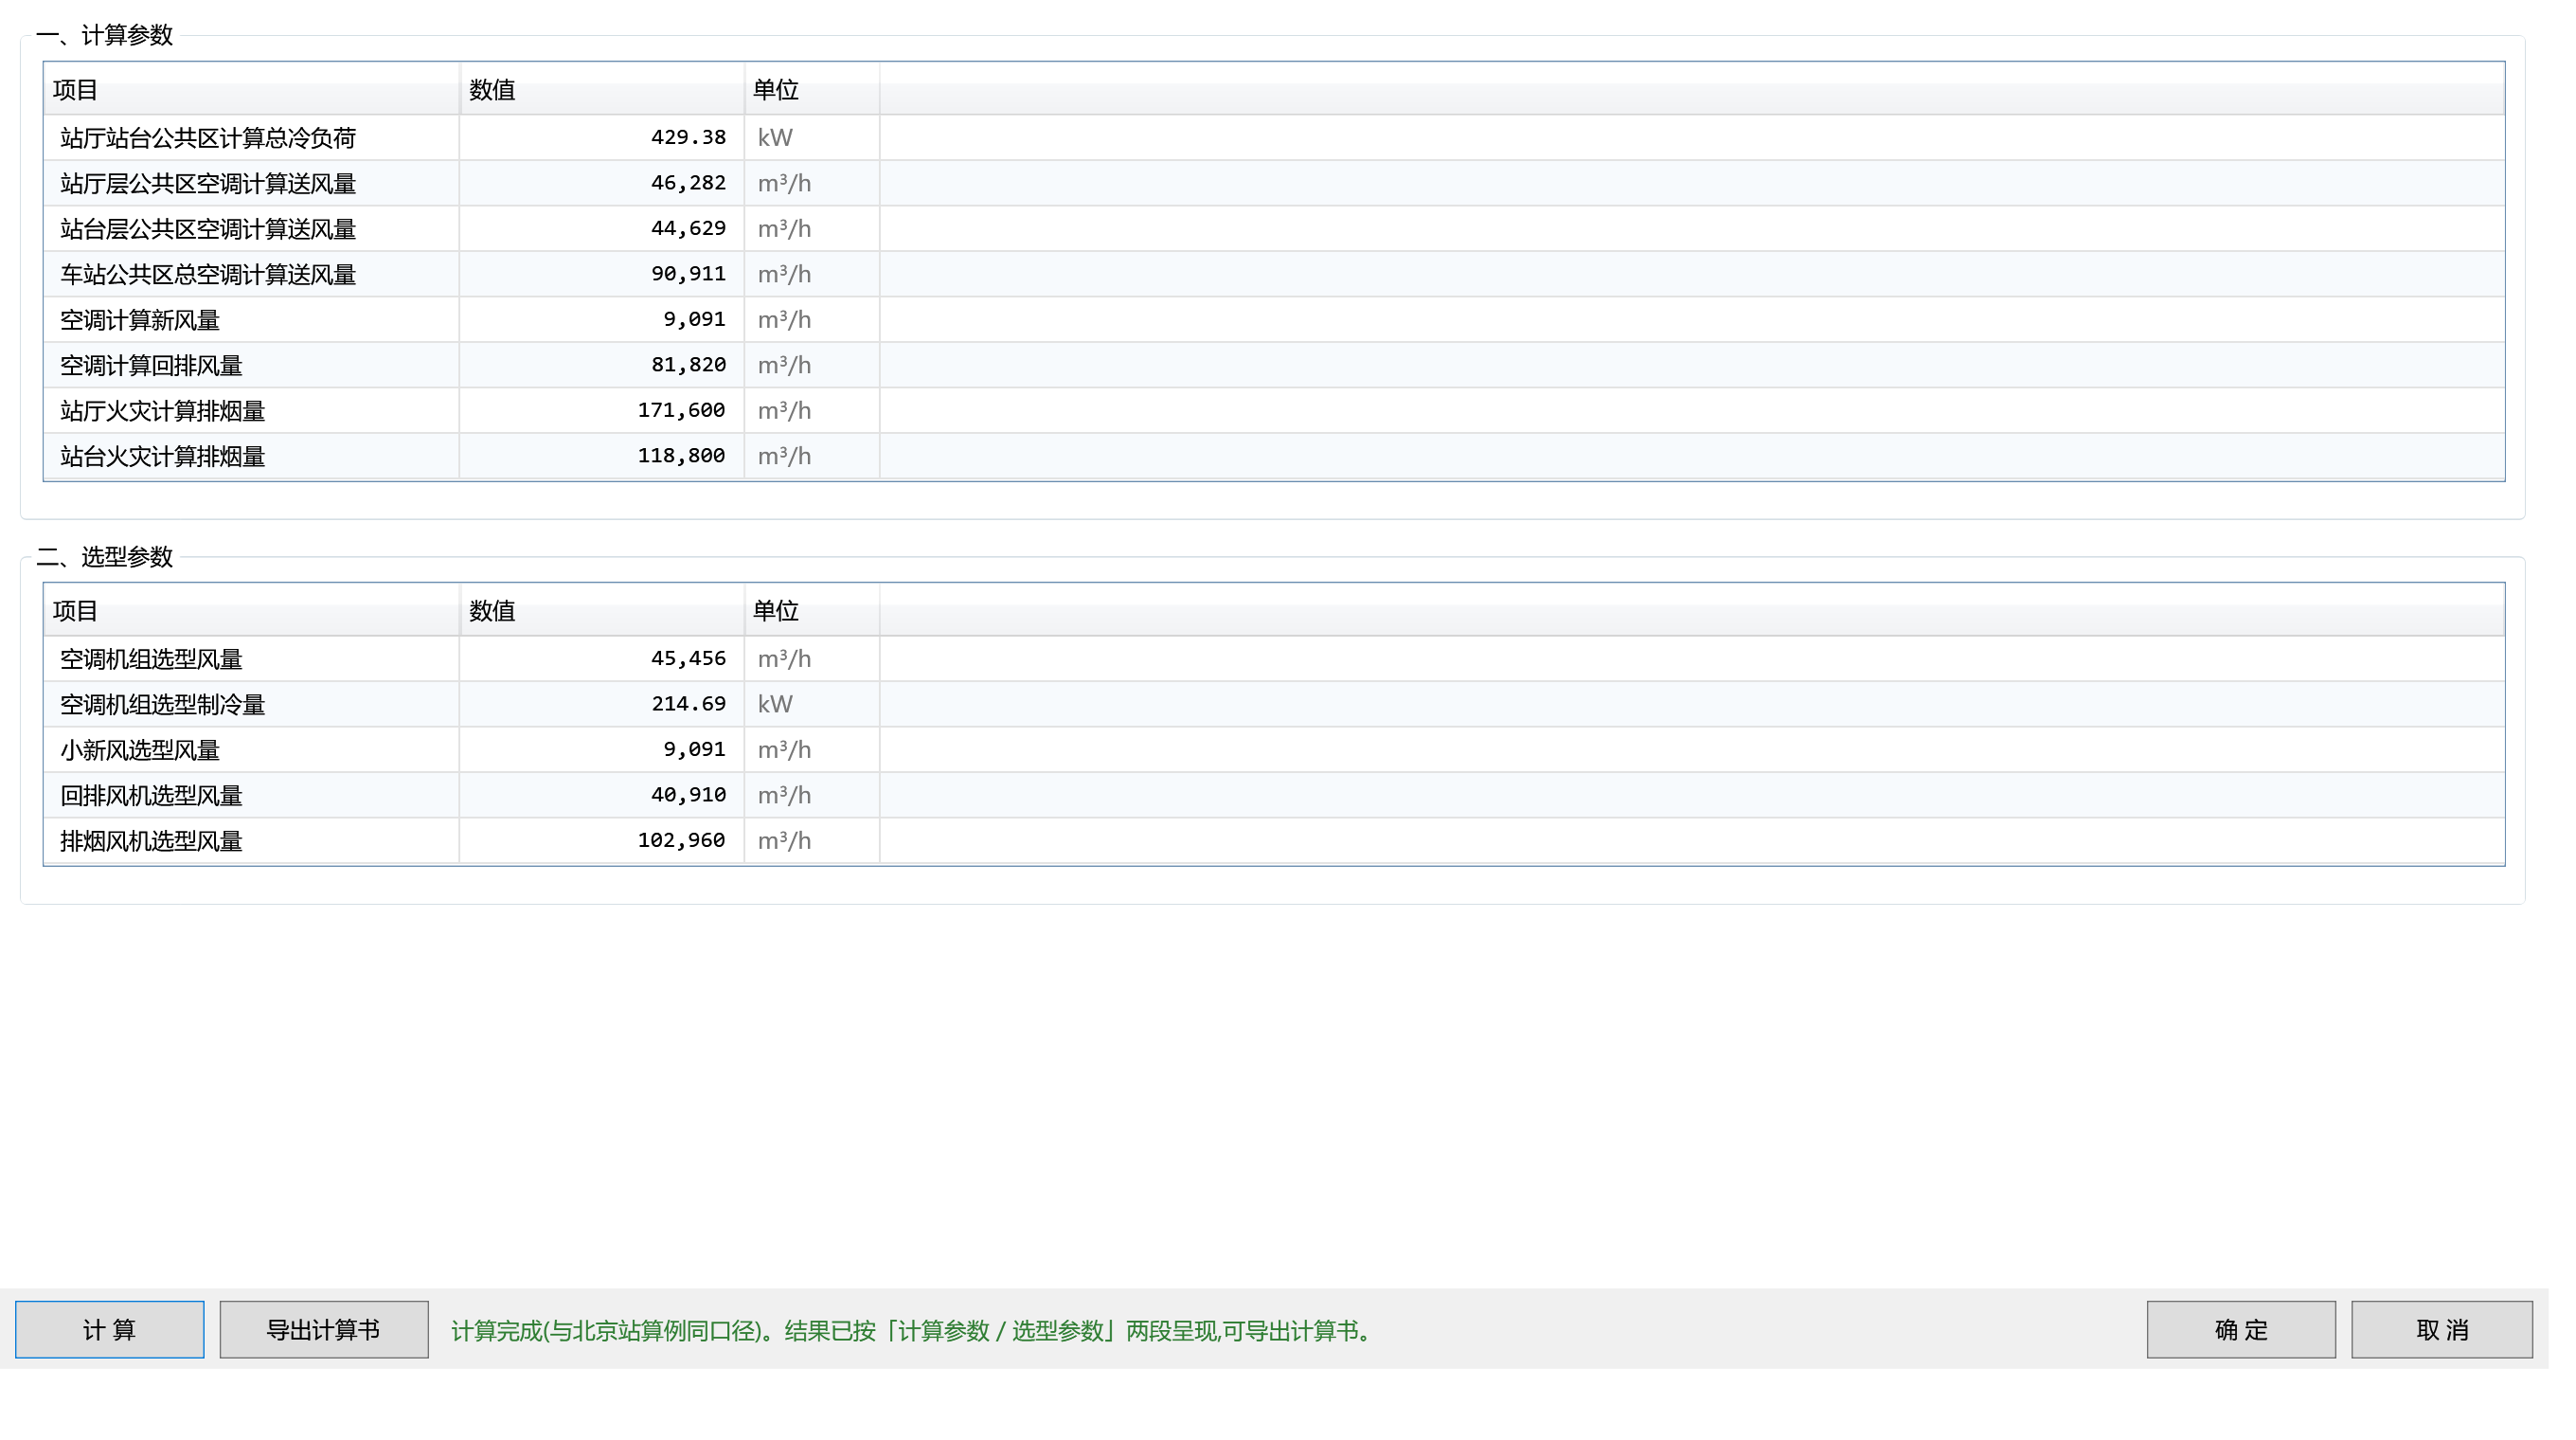
\includegraphics[width=0.95\textwidth]{figures/large-result.png}
\caption{大系统计算结果窗:计算参数与选型参数}\label{fig:calc}
\end{figure}

\begin{figure}[H]
\centering
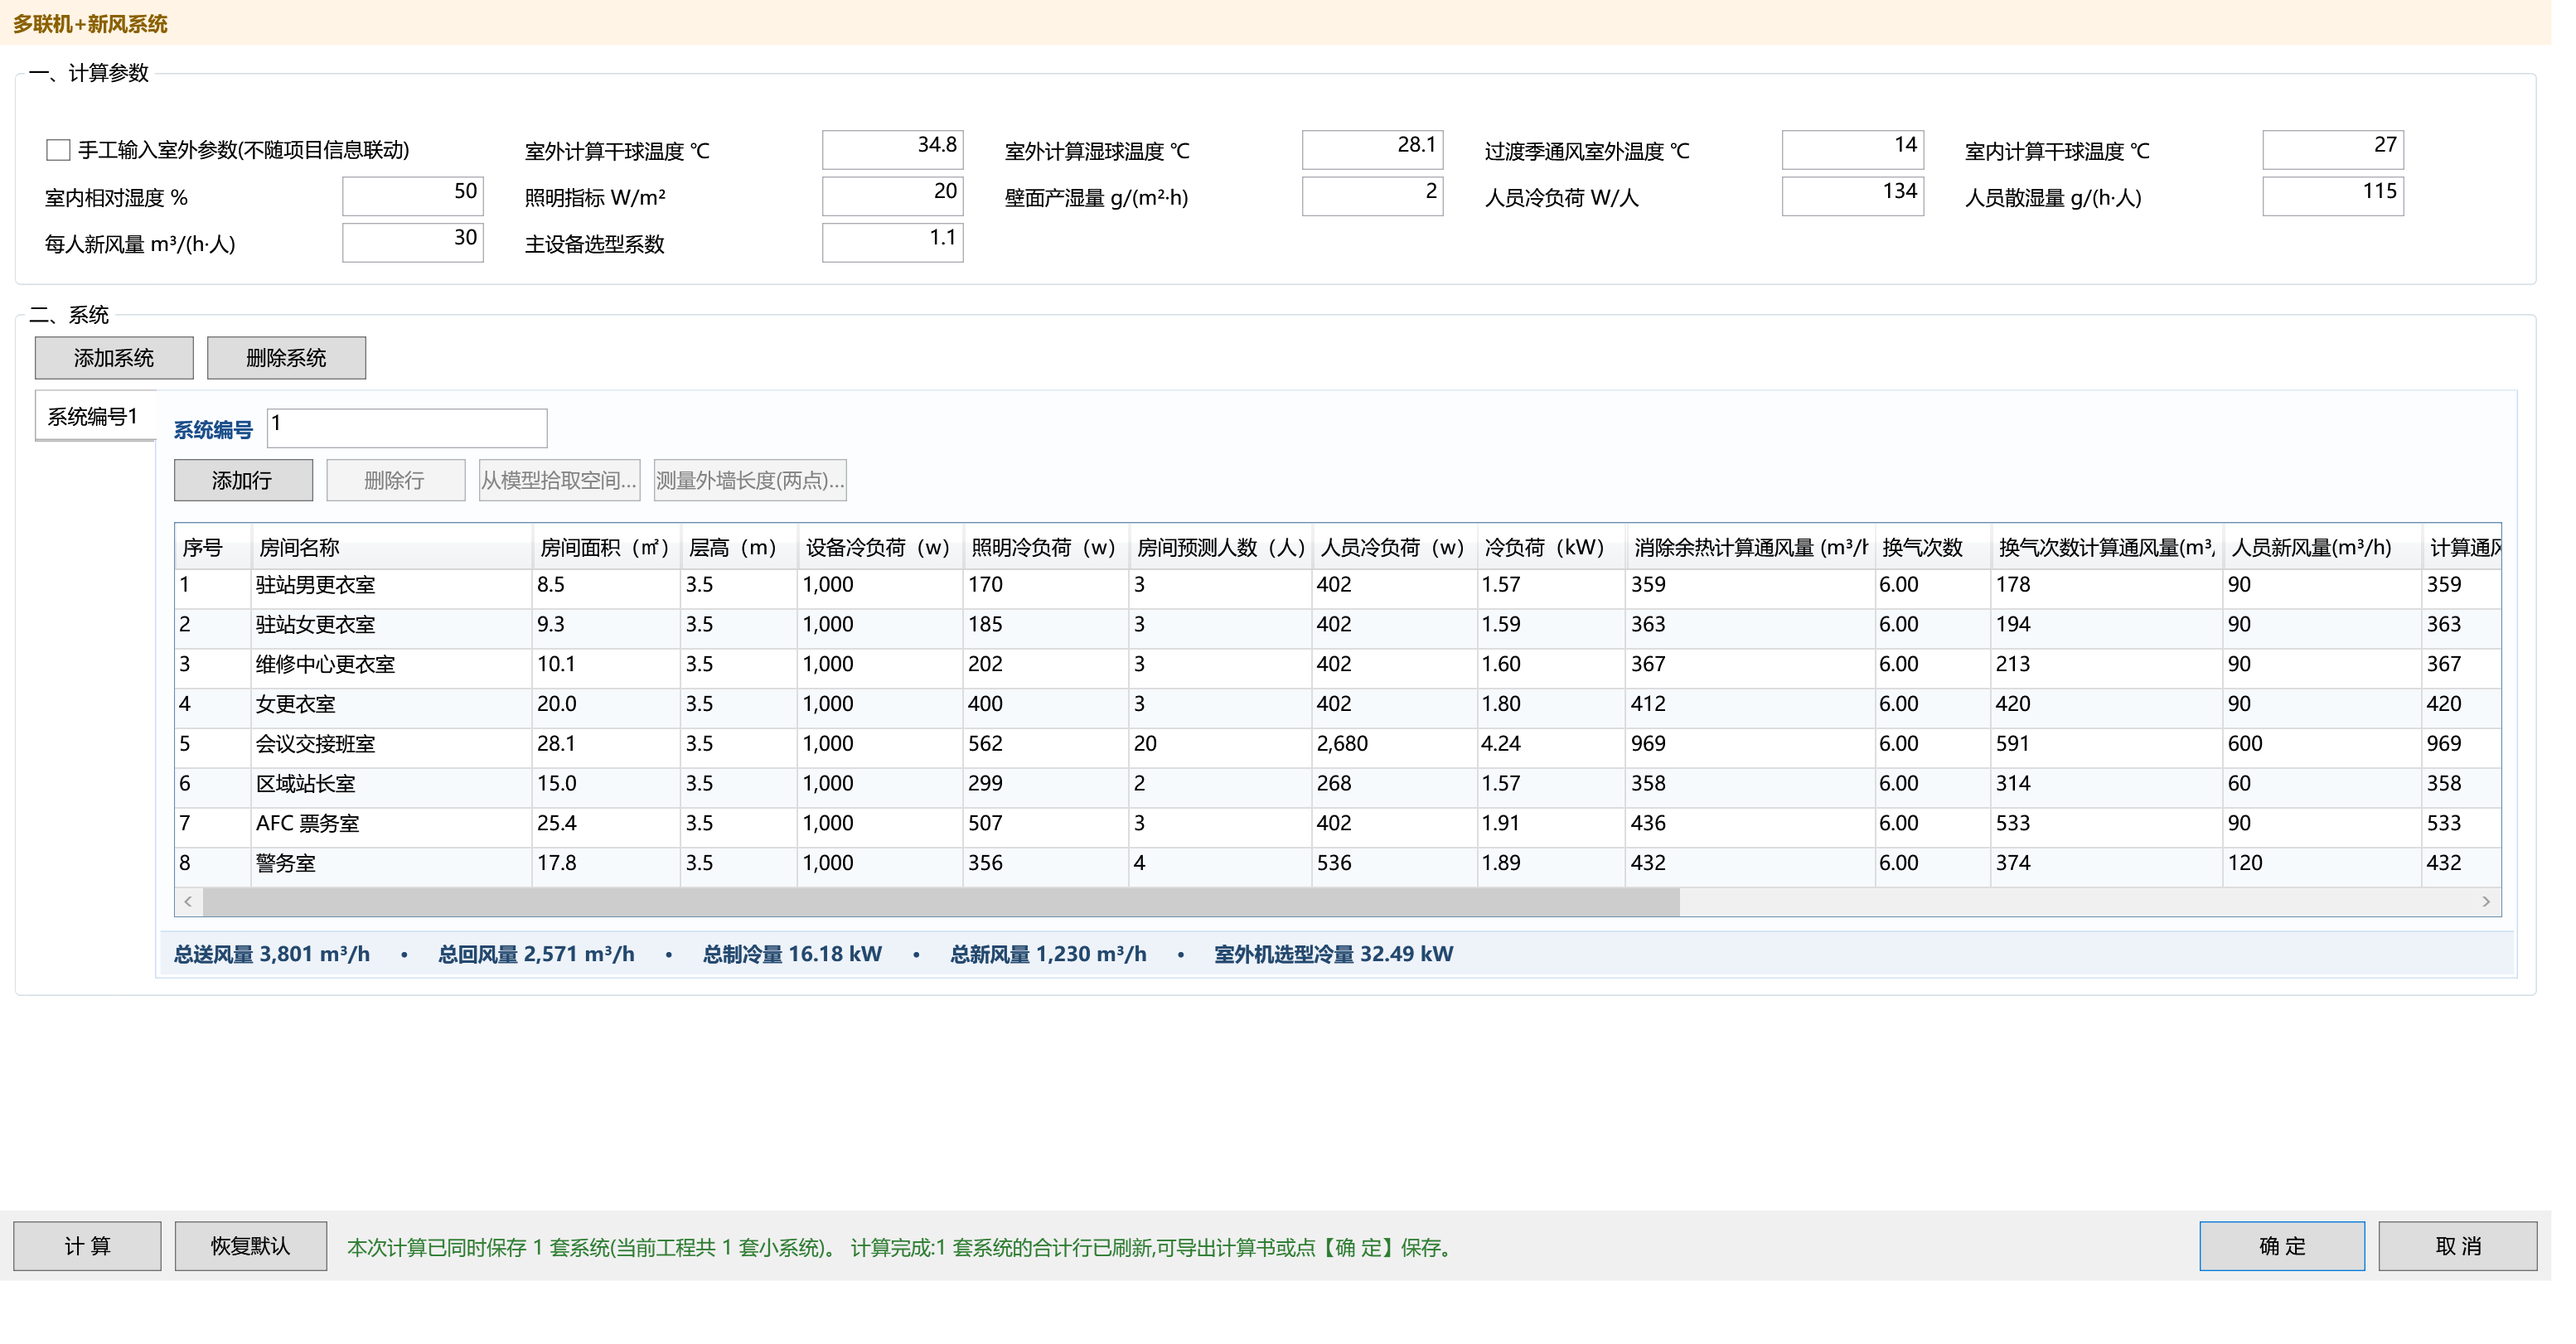
\includegraphics[width=0.95\textwidth]{figures/small-vrf.png}
\caption{多联机+新风系统房间表(20 列,前段可编辑、后段自动计算)}\label{fig:vrf}
\end{figure}

\subsection{数值验证}

大系统以北京站算例为回归输入,总制冷量 381.598 kW、总送风量 87\,768 m$^3$/h 与工作簿一致;剔除由项目信息联动补入的气象三格后,其余各格同样一致。小系统六类分别以文档示例复算(表\ref{tab:cases}):全空气一次回风的空调器冷量合计 162.2 kW,示例为 157.6 kW,差约 3\%,原因是示例中部分房间按消除余热通风量取值,而正文规定按计算通风量取值——差异写进规则说明,断言只锚正文。

\begin{table}[H]
\centering
\caption{六类小系统的回归算例与关键量}\label{tab:cases}
\small
\begin{tabular}{p{2.6cm}p{5.6cm}p{4.6cm}}
\toprule
系统类型 & 算例规模 & 关键校核量 \\
\midrule
全空气一次回风 & 21 个房间 & 冷负荷 104.42 kW;送风 32\,539 m$^3$/h;空调器冷量 162.2 kW \\
多联机+新风 & 11 个房间(选型另按 7 房间示例) & 冷负荷 21.57 kW;室外机选型 27.3184 kW \\
排风 & 8 个房间 & 计算排风量 5\,386 m$^3$/h \\
排烟 & 2 个防烟分区 & 计算排烟 34\,620 m$^3$/h;补风 20\,772 m$^3$/h \\
送风排风排烟 & 5 个房间 & 排风 20\,307、排烟 31\,020、补风 18\,612 m$^3$/h \\
加压送风 & 楼梯间门参数 & 加压送风量 14\,412.4 m$^3$/h \\
\bottomrule
\end{tabular}
\end{table}

\subsection{与单点工具的对比}

表\ref{tab:compare} 从工具链的五个环节对比三种做法。单点工具并非"更差",而是在"环节内效率"与"环节间传递"之间做了不同取舍;本工具链牺牲了一部分灵活性,换取改动只发生一次。

\begin{table}[H]
\centering
\caption{单点工具与工具链的对比}\label{tab:compare}
\small
\begin{tabular}{p{2.4cm}p{3.8cm}p{3.8cm}p{4.6cm}}
\toprule
环节 & Excel 表格 & 通用 BIM 插件 & 本工具链 \\
\midrule
取数 & 人工抄录 & 模型取值 & 模型取值 + 来源 Id 追溯 \\
规则 & 分散在工作簿 & 引擎内置,不可见 & 文档逐条移植,可对照 \\
计算 & 公式即表 & 通用算法 & 六类 + 大系统 + 水力,可测 \\
交付 & 手工整理 & 部分导出 & 计算书/材料表/图册一致 \\
回归 & 无 & 弱 & 900+ 条断言 \\
\bottomrule
\end{tabular}
\end{table}

\section{讨论}

\paragraph{工具链的瓶颈在规则,不在算法。}
负荷、排烟、水力都是成熟公式,算法本身没有难点;难点在于"院内的规则到底是什么、写在哪、和示例冲突时听谁的"。规则建模做不扎实,后面的自动化只是把错误算得更快。因此本工具链把第一环的产出(常量、默认值、校核值)当作与代码同等重要的交付物。

\paragraph{输出一致是交付的验收条件。}
计算书交付出去,评审不会只问"数对不对",还会问"这个数和界面上的是不是一回事"。一致输出让这个问题不再需要回答:三处读同一份对象,差异只可能来自格式,不可能来自计算。反过来,若各出口各自计算,即便每个都对,也解释不清"为什么不一样"。

\paragraph{迁移成本与局限。}
工具链的代价是前期投入:规则要逐条落实,约定要设计,自动检查要写。对一个站、一类系统,这些投入未必划算;对多站、多专业复用的设计院,才会回本。局限有三:公式随文档漂移,需要版本化基线;模型取值依赖空间已放置且已计算体积;仅在 Revit 2020 上验证,高版本 API 差异(如单位制接口)尚未覆盖。

\section{结论}

本文把地铁暖通的正向设计作业链作为整体,构建了一条由规则建模、模型取值、计算内核、一致输出、交付生成五环组成的工具链,并以数据约定与三道自动检查保证环节之间不断裂。北京站算例与六类小系统示例的逐格校核表明,工具链的关键计算结果与院内工作簿一致;工程应用表明,设计人可以把精力从"抄数与整理"转向"判断与选型"。工具链的价值不在单点更强,而在改动只发生一次——这正是"正向"二字在工程软件里的具体含义。后续工作将围绕高版本 Revit 适配、选型结果回写模型,以及把规则基线纳入版本管理展开。

\begin{thebibliography}{9}
\bibitem{taghaddos2019} Taghaddos H, Mashayekhi A, Sherafat B. Automation of construction quantity take-off: using building information modeling (BIM)[J]. arXiv preprint arXiv:1906.02400, 2019.
\bibitem{noardo2020} Noardo F, Wu T, Arroyo Ohori K, et al. IFC models for (semi)automating common planning checks for building permits[J]. arXiv preprint arXiv:2011.03117, 2020.
\bibitem{quinn2022} Quinn C, Zargar Shabestari A, Litoiu M, et al. Building automation system data integration with BIM: data structure and supporting case study[J]. arXiv preprint arXiv:2205.05518, 2022.
\bibitem{dang2024ahmsys} Dang L H, Nguyen D H, Le T Q, et al. AHMsys: an automated HVAC modeling system for BIM project[J]. arXiv preprint arXiv:2407.01987, 2024.
\bibitem{revitapi2020} Autodesk. Revit 2020 API developer guide[EB/OL]. https://www.autodesk.com/developer-network/platform-technologies/revit, 2019.
\bibitem{gb50736} 中华人民共和国住房和城乡建设部. 民用建筑供暖通风与空气调节设计规范: GB 50736—2012[S]. 北京: 中国建筑工业出版社, 2012.
\bibitem{gb50157} 中华人民共和国住房和城乡建设部. 地铁设计规范: GB 50157—2013[S]. 北京: 中国建筑工业出版社, 2013.
\end{thebibliography}

\end{document}
